\label{chap:exact-methods}
Despite the promising results achievable with a well-designed heuristic, it is necessary to consider strategies aimed at finding the optimal solutions.

Before going into the implementation of exact methods, we must first examine the problem formulation introduced in Section~\ref{sec:prob-form}, particularly the Subtour Elimination Constraints (SECs) in Equation~\ref{eq:ilp_sec}. It is important to highlight that the number of SECs grows exponentially with respect to the number of nodes in the instance, making it infeasible to generate all of them upfront, even for problems of moderate size.

This section presents the implementation of exact methods whose goal is to generate SECs in a more intelligent and efficient manner, leveraging CPLEX to solve the resulting mathematical model.

\section{CPLEX}

CPLEX is a high-performance solver for linear programming (LP), mixed-integer programming (MIP), and quadratic programming problems. It is widely used in both academic research and industrial applications due to its efficiency, scalability, and support for advanced solving techniques. \cite{cplex2023}

It provides a rich set of APIs, allowing for integration into custom optimization workflows, along with powerful features like presolving, cutting planes, heuristics, and branch-and-bound algorithms. One of the most useful functionalities of CPLEX for combinatorial optimization problems, such as the Traveling Salesman Problem, is the support for \emph{callbacks}. These allow users to interact with the solver during the optimization process, for example, by adding constraints dynamically (lazy constraints) or customizing branching decisions.

In this work, CPLEX is used to solve the integer linear programming (ILP) formulation of the TSP, taking advantage of its support for dynamic constraint generation to efficiently handle the exponential number of Subtour Elimination Constraints.

\section{Benders Decomposition}

Benders Decomposition is a general technique for solving large-scale mixed-integer problems by iteratively decomposing them into a master problem and one or more subproblems. 

In our implementation, the main idea is to:
\begin{itemize}
    \item Solve a relaxed version of the ILP model without SECs.
    \item Analyze the resulting solution to detect subtours (disconnected components).
    \item Add one or more SECs to eliminate these subtours.
    \item Repeat the process until a connected solution is found.
\end{itemize}

\begin{figure}[H]
    \centering
    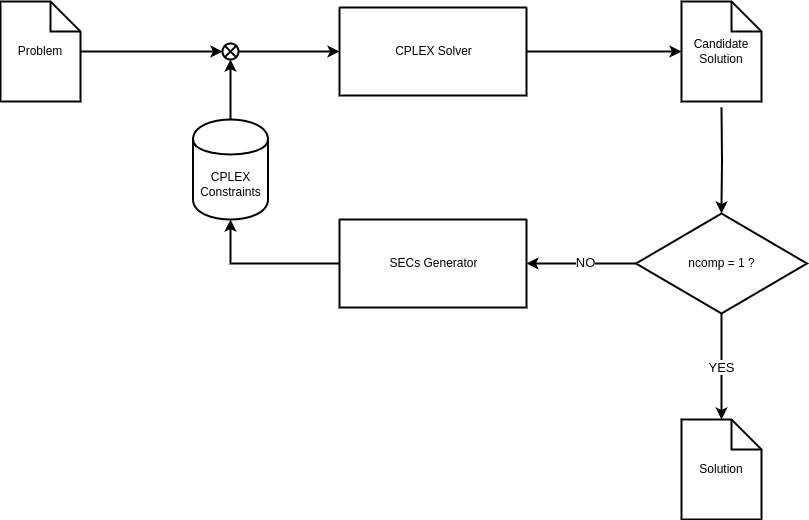
\includegraphics[width=0.9\textwidth]{benders_flow.drawio.png}
    \caption{Flowchart of the Benders-like solving loop for the TSP.}
    \label{fig:benders_flowchart}
\end{figure}

\subsection{Cycle Detection and SEC Addition.}
The solution provided by CPLEX after each iteration is typically fractional or disconnected. To restore feasibility, we apply a component detection procedure: all edges \( x_{ij} \) such that \( x_{ij} > 0.5 \) are considered part of the current solution, and a union-find-like structure is used to identify the connected components.

For each component \( C_k \), we add the following constraint:
\[
\sum_{\substack{i,j \in C_k \\ i \neq j}} x_{ij} \leq |C_k| - 1
\]
This ensures that in future iterations, such subtours will be avoided.

\subsection{Pseudocode}
\begin{algorithm}[H]
\caption{Subtour Elimination Loop}
\begin{algorithmic}[1]
\State Initialize \texttt{comp[i] = -1} for all nodes $i$, and set \texttt{ncomp = 0}
\Repeat
    \State Solve the relaxed ILP using \texttt{CPXmipopt}
    \State Extract solution and build components from $x^*_{ij} > 0.5$
    \State \texttt{ncomp} $\gets$ number of connected components
    \If{$ncomp > 1$}
        \For{each component $C_k$}
            \State Add SEC: $\sum_{i,j \in C_k} x_{ij} \leq |C_k| - 1$
        \EndFor
    \EndIf
\Until{\texttt{ncomp} = 1 or time limit reached}
\end{algorithmic}
\end{algorithm}

The entire loop is managed manually, CPLEX is invoked multiple times, at each iteration with an updated model that includes new constraints.

\subsection{Patching Heuristic}
\label{ssec:patching}
In cases where the solving loop exceeds the time limit or fails to converge to a single connected component, we introduce a fallback heuristic called \emph{patching}, which aims to merge disconnected subtours into a feasible Hamiltonian cycle.

The algorithm works as follows:
\begin{itemize}
    \item Identify all components (subtours) in the current solution.
    \item For each pair of components, consider removing an edge from one component and connecting its endpoint to a node in the other component.
    \item Compute the extra cost for each reconnection and select the pair that minimizes the increase in total cost.
    \item Repeat the operation until all components are merged into a single tour.
\end{itemize}

\begin{figure}[H]
    \centering
    \begin{subfigure}{0.45\textwidth}
        \centering
        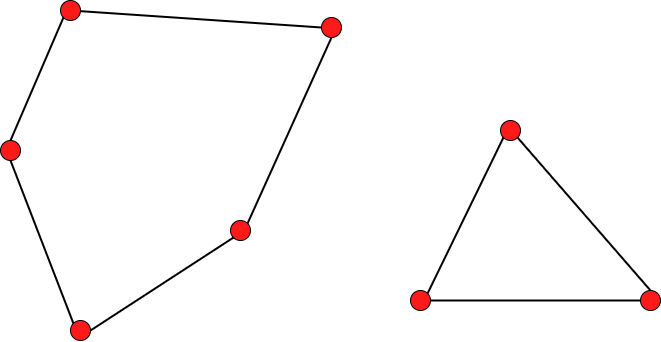
\includegraphics[width=\textwidth]{pre_patch.drawio.png}
        \caption{Disconnected subtours (MIP solution)}
        \label{fig:pre_patch}
    \end{subfigure}
    \hfill
    \begin{subfigure}{0.45\textwidth}
        \centering
        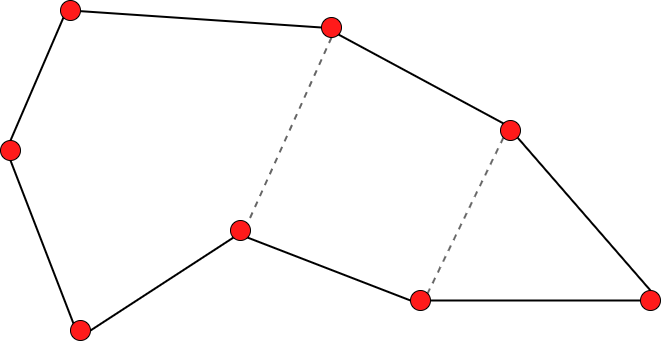
\includegraphics[width=\textwidth]{post_patch.drawio.png}
        \caption{Final tour after patching}
        \label{fig:post_patch}
    \end{subfigure}
    \caption{Visual example of the patching heuristic. The initial MIP solution contains multiple disconnected cycles (a), which are then merged into a single feasible tour (b) using edge reconnection.}
    \label{fig:patching_combined}
\end{figure}

Finally, once a patched tour is constructed, a local optimization phase (e.g., 2-opt) can optionally be applied to refine the solution quality. Obviously, this solution does not guarantee optimality, but it is a reliable fallback in case the Benders loop does not have enough time to reach the global minimum.

\section{Branch-and-Cut}

Branch-and-Cut is a state-of-the-art exact method for solving the TSP and many other combinatorial problems. It extends the classical Branch-and-Bound algorithm by dynamically adding valid inequalities (cuts) to the model, such as Subtour Elimination Constraints, during the exploration of the branch-and-bound tree.

In our implementation, we leverage CPLEX’s built-in support for lazy constraint callbacks to detect and eliminate subtours on-the-fly. This allows us to start from a relaxed ILP formulation and enforce connectivity only when needed, without pre-generating the exponential number of SECs.

\subsection{Lazy Constraint Mechanism}

Rather than rebuilding the model after each solution, Branch-and-Cut integrates subtour elimination directly into the solving loop through a callback mechanism. After each integer-feasible solution is identified by the solver, a callback is triggered to verify whether the current edge selection forms a valid Hamiltonian cycle. This is achieved by analyzing the connected components of the solution. If multiple subtours are found, one or more violated SECs are generated and dynamically injected into the model as lazy constraints.

This logic can be visualized using the flow in Figure~\ref{fig:benders_flowchart}, with the only difference being that SECs are injected directly into the CPLEX solver, and the model is not rebuilt from scratch at each iteration.

This interaction happens entirely within the solver, reducing overhead and fully exploiting CPLEX’s branch-and-bound engine. In our implementation, this is realized by registering a lazy constraint callback under the candidate solution context, which ensures that only integer-feasible solutions are inspected. The integration is fully transparent to the solver's internal mechanisms, preserving performance.

\subsection{Pseudocode}

\begin{algorithm}[H]
\caption{Callback-based Subtour Elimination}
\begin{algorithmic}[1]
\State Define lazy constraint callback function:
\Statex \quad Extract $x^*_{ij}$ from current solution
\Statex \quad Build connected components from $x^*_{ij} > 0.5$
\If{\texttt{ncomp} $>$ 1}
    \For{each component $C_k$}
        \State Add SEC: $\sum_{i,j \in C_k} x_{ij} \leq |C_k| - 1$
    \EndFor
\EndIf
\State Attach callback to CPLEX model
\State Solve the ILP using \texttt{CPXmipopt}
\end{algorithmic}
\end{algorithm}

The callback logic relies on identifying connected components from the edge variables $x_{ij}$ using a simple traversal procedure. Subtours are detected efficiently and corresponding SECs are added using CPLEX's lazy constraint API, avoiding the need to rebuild the model.

This structure ensures that any subtour detected during the search is immediately eliminated, allowing the solver to explore only feasible (or corrected) branches.
